\documentclass[danish,a4paper]{report}
\usepackage[T1]{fontenc}
\usepackage[utf8]{inputenc}
\usepackage{lmodern}
\usepackage{hyperref}
\usepackage{graphicx}
\usepackage[english]{babel}
\usepackage{verbatim}
\usepackage{color}
\usepackage[table]{xcolor}
\usepackage{graphicx}

\usepackage{tikz}
\usetikzlibrary{automata,positioning}

\usepackage{parskip}
\usepackage{url}
\usepackage{background}
\usepackage{lastpage}
\usepackage{titlesec}
\usepackage{blindtext}
\usepackage{color}
\usepackage{nopageno}
\usepackage{todonotes}
\usepackage{listings}

\definecolor{dkgreen}{rgb}{0,0.6,0}
\definecolor{gray}{rgb}{0.5,0.5,0.5}
\definecolor{mauve}{rgb}{0.58,0,0.82}
\definecolor{gray75}{gray}{0.75}
\definecolor{light-gray}{gray}{0.5}

\lstset{
  frame=,
  language=C,
  aboveskip=3mm,
  belowskip=3mm,
  showstringspaces=false,
  columns=flexible,
  basicstyle={\small\ttfamily},
  numbers=none,
  numberstyle=\tiny\color{gray},
  keywordstyle=\color{blue},
  commentstyle=\color{dkgreen},
  stringstyle=\color{mauve},
  breaklines=true,
  breakatwhitespace=true
  tabsize=4
}

\addtolength{\topmargin}{-1.5cm}
\addtolength{\textheight}{1.5cm}
\addtolength{\oddsidemargin}{-1cm}
\addtolength{\evensidemargin}{-1cm}
\addtolength{\textwidth}{2cm}

 
\definecolor{schultz}{RGB}{146,34,126}
\definecolor{gray75}{gray}{0.75}
\definecolor{light-gray}{gray}{0.5}
\newcommand{\hsp}{\hspace{20pt}}
\titleformat{\chapter}[hang]{\Huge\bfseries}{\thechapter\hsp}{0pt}{\Huge\bfseries}[{\titlerule[1.5pt]}]
% \titlespacing*{\chapter}{0cm}{-10pt}{2em}
\titlespacing*{\chapter}{0cm}{-20pt}{2em}
\setcounter{secnumdepth}{3}
\setcounter{tocdepth}{1}

\titlespacing*{\section} {0pt}{5pt}{2pt}
\titlespacing*{\subsubsection}{0pt}{0pt}{0pt}

\backgroundsetup{
  scale=1,
  color=black,
  opacity=1,
  angle=0,
  position=current page.south,
  vshift=60pt,
  contents={%
  \small%
  \begin{minipage}{.48\textwidth}
  \vspace{-2cm}
  \parbox[b]{.4\textwidth}{%
    Side \thepage\ af \pageref{LastPage}}\hfill
  \parbox[b]{.6\textwidth}{%
  \raggedleft \titlename}
  \rule{\textwidth}{1.5pt}\\
  \parbox[b]{.7\textwidth}{%
      \name }\hfill
  \parbox[b]{.3\textwidth}{%
  \raggedleft \email } 
  \end{minipage}\hspace{.02\textwidth}%
  \begin{minipage}{.5\textwidth}
  \vspace{-2cm}
  \includegraphics[width=\linewidth,height=70pt,keepaspectratio]{footer_logo}
  \end{minipage}%
  }
}

\newcommand{\namesigdate}[2][10cm]{%
  \begin{tabular}{@{}p{#1}@{}}
    #2 \\[2\normalbaselineskip] \hrule \\[0pt]
    {\small \textit{Signature}} \\[2\normalbaselineskip] \hrule \\[0pt]
    {\small \textit{Date}}
  \end{tabular}
}

\newcommand{\titlename}{Programmer som Data}
\newcommand{\name}{Jacob Benjamin Cholewa}
\newcommand{\email}{jbec@itu.dk}


\makeatletter
\NoBgThispage
 \title{\Huge \textbf{\titlename}\\\huge Eksamens opgave Januar 2015}
 % Author
\author{\textsc{\name} \\ \textsc{\email}}
\begin{document}
\maketitle

\vspace*{\fill}
\begin{center}
\begin{large}
Jeg erklærer hermed at jeg selv har lavet hele denne eksamensbevarelse uden hjælp fra andre
\end{large}

\vspace*{2cm}
\namesigdate{}
\end{center}

\vspace*{\fill}


\newpage

\chapter*{Opgave 1}
\section*{Spørgsmål 1}
Det regulære udtryk $e(fd*)*x$ beskriver et bar system. Du kan gå ind i baren, $e(nter)$, og her kan du så hente øl, $f(etch)$, (Du behøver ikke). Når du har en øl kan du hente en mere eller du kan drikke af den du allerede har 0 til flere gange $d(rink)$. Tilsidst kan du gå ud af baren, $e(xit)$, lige gyldigt om du har eller ikke har hentet og drukket øl.

Dette regulære udtryk beskriver altså for eksempel disse strenge:
\begin{center}$ ex$,
$efx$,
$effx$,
$efdx$,
$efffdx$,
$efddfddfx$
\end{center}
hvor disse strenge ville være ugyldige:
\begin{center}
$fx$,
$fdx$,
$efd$,
$edx$
\end{center}
\section*{Spørgsmål 2}
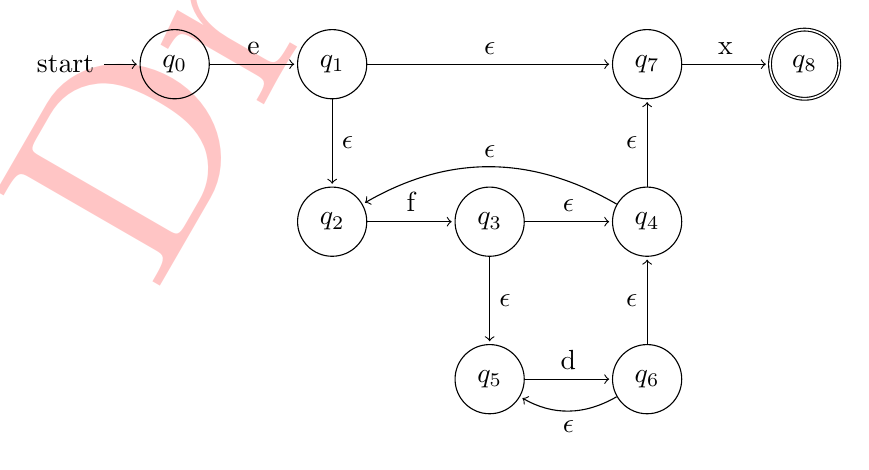
\begin{tikzpicture}[shorten >=1pt,node distance=2cm,on grid,auto] 
   \node[state,initial]   (q_0)                         {$q_0$}; 
   \node[state]           (q_1) [right=of q_0]          {$q_1$};
   \node[state]           (q_2) [below=of q_1]          {$q_2$}; 
   \node[state]           (q_3) [right=of q_2]          {$q_3$}; 
   \node[state]           (q_4) [right=of q_3]          {$q_4$}; 
   \node[state]           (q_5) [below=of q_3]          {$q_5$}; 
   \node[state]           (q_6) [right=of q_5]          {$q_6$}; 
   \node[state]           (q_7) [above=of q_4]          {$q_7$}; 
   \node[state,accepting] (q_8) [right=of q_7]          {$q_8$}; 


    \path[->] 

    (q_0) edge              node {e}           (q_1)
    (q_1) edge              node {$\epsilon$}  (q_7)
          edge              node {$\epsilon$}  (q_2)
    (q_2) edge              node {f}           (q_3)
    (q_3) edge              node {$\epsilon$}  (q_4)
          edge              node {$\epsilon$}  (q_5)
    (q_4) edge              node {$\epsilon$}  (q_7)
          edge [bend right] node [swap ]{$\epsilon$}  (q_2)
    (q_5) edge              node {d}           (q_6)
    (q_6) edge [bend left]  node {$\epsilon$}  (q_5)
          edge              node {$\epsilon$}  (q_4)
    (q_7) edge              node {x}           (q_8);
\end{tikzpicture}

\section*{Spørgsmål 3}
\begin{table}[h]
\centering
\begin{tabular}{|l|l|l|l|l|l|}
\hline
State      & e   & f   & d   & e      & NFA States                            \\ \hline
$S_0$      & $S_1$  & -      & -      & -     & $\{q_0\}$                     \\
$S_1$      & -      & $S_3$  & -      & $S_2$ & $\{q_1, q_2, q_7\}$           \\
$S_2$      & -      & -      & -      & -     & $\{q_8\}$                     \\
$S_3$      & -      & $S_3$  & $S_4$  & $S_2$ & $\{q_2, q_3, q_4, q_5, q_7\}$ \\
$S_4$      & -      & $S_3$  & $S_4$  & $S_2$ & $\{q_2, q_4, q_5, q_6, q_7\}$ \\ \hline
\end{tabular}
\end{table}

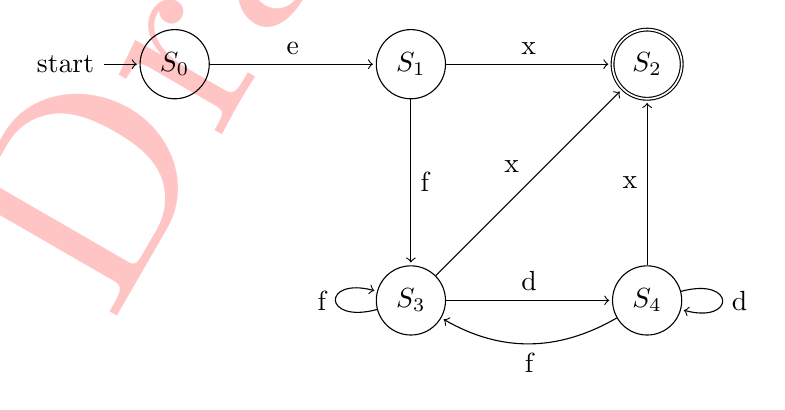
\begin{tikzpicture}[shorten >=1pt,node distance=3cm,on grid,auto] 
   \node[state,initial]   (s_0)                         {$S_0$}; 
   \node[state]           (s_1) [right=of s_0]          {$S_1$};
   \node[state,accepting] (s_2) [right=of s_1]          {$S_2$}; 
   \node[state]           (s_3) [below=of s_1]          {$S_3$}; 
   \node[state]           (s_4) [right=of s_3]          {$S_4$}; 


    \path[->] 

    (s_0) edge                node          {e} (s_1)
    (s_1) edge                node          {x} (s_2)
          edge                node          {f} (s_3)
    (s_3) edge  [loop left]   node          {f} (s_3)
          edge                node          {d} (s_4)
          edge                node          {x} (s_2)
    (s_4) edge  [loop right]  node          {d} (s_4)
          edge  [bend left]   node          {f} (s_3)
          edge                node          {x} (s_2)
          ;

\end{tikzpicture}
\section*{Spørgsmål 4}

\label{LastPage}
\end{document}